%\subsection{Testing testing...}
This is where the testing results go

some numbers for now: Transfers running since March, some 2.6 million transfers, 87\% success
rate, over 2 PB of data so far. This is approximately 7\% of the rate CMS achieves globally.

% Points to make:
We used the PhEDEx LifeCycle agent \cite{LifeCycle} to drive transfers between pairs of sites, using gridftp with the IPv6 connectivity flags. Filesizes were checked at the destination, and any failures recorded. Files were transferred in both directions between each site pair.

Initially, we simply tested connectivity and basic functionality. We also tested under specific conditions, e.g. to compare throughput and error rates with IPv6 vs. IPv4 connectivity. This was useful for debugging issues with firewalls etc.

Since March 2013 the transfer testbed has been running continuously, with more sites joining over time. Finally we have 11 sites transferring 1 GB files between each other. With this many sites, we have had to introduce a delay between successive transfers, to reduce load on the servers.

To date, we have transferred over 2 PB of data between the 11 sites over the 6 months since the testbed started continuous operations. This is 7\% of the rate that CMS achieve in daily operations, so not an insignificant amount. The overall success rate for transfers is 87\%, which is very high considering that the testbed was operated at-risk, with errors only detected when someone decided to look for them.

% 2.6 M transfers, 87\% success, over 2 PB transferred, which is ~ 7\% of global CMS rate
See figure \ref{fig:full-mesh} for the full mesh.

% discuss results of figure full-mesh

% PhEDEx transfers. using private PhEDEx instance and nodes. DPM and FTS3. Transfers throttled to avoid overload. PhEDEx now shown to run with IPv6 endpoints.
% Simon/Duncan to describe this bit better

% To create this graphic:
% 1) save your image as a 1024x1024 png/gif/bmp
% 2) convert to pdf (install ImageMagick, then 'convert FileIn.png FileOut.pdf')
% N.B. if the input and output files have the same base name, LaTeX will prefer to take the png over the pdf,
% which is probably not what you want. Make sure the files have different names!
\begin{figure}[htp]
\centering
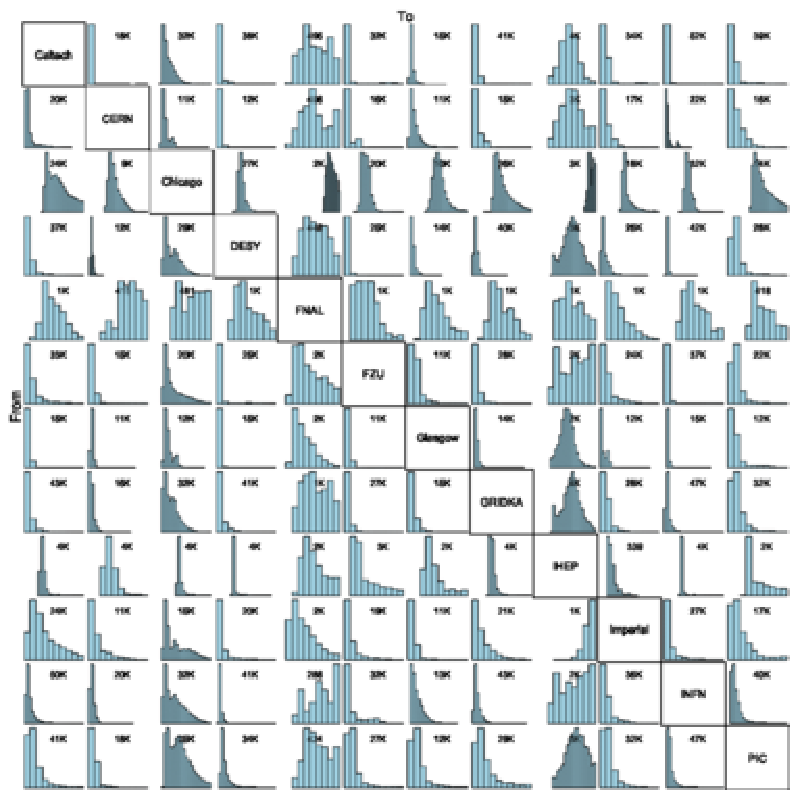
\includegraphics{full-mesh}
\caption{Transfer performance for the IPv6 testbed continuous transfers. A 1 GB file is transferred between each pair of sites, then deleted, then transferred again, continuously. The plots show the distribution of transfer duration times per site pair. The source site is named in the row, the destination site is named in the column. So the top-right plot shows transfers from Caltech to PIC, the bottom-left shows transfers fromPIC to Caltech. The x-axis is in seconds, from 0 to 500 for each plot. The number inset in each plot shows the approximate number of transfers between that site pair in that direction.}\label{fig:full-mesh}
\end{figure}

\begin{figure}[htp]
\centering
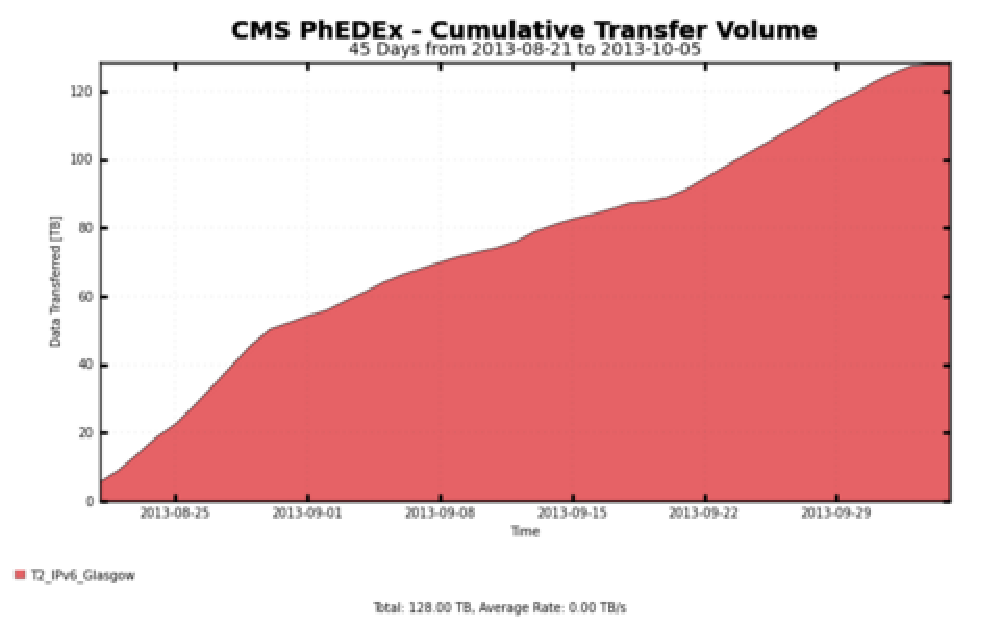
\includegraphics{phedex-transfer-volume}
\caption{Cumulative data-transfer between Imperial College and Glasgow using PhEDEx on the IPv6 testbed.}\label{fig:phedex-transfer-volume}
\end{figure}

